%
% File acl2020.tex
%
%% Based on the style files for ACL 2020, which were
%% Based on the style files for ACL 2018, NAACL 2018/19, which were
%% Based on the style files for ACL-2015, with some improvements
%%  taken from the NAACL-2016 style
%% Based on the style files for ACL-2014, which were, in turn,
%% based on ACL-2013, ACL-2012, ACL-2011, ACL-2010, ACL-IJCNLP-2009,
%% EACL-2009, IJCNLP-2008...
%% Based on the style files for EACL 2006 by 
%%e.agirre@ehu.es or Sergi.Balari@uab.es
%% and that of ACL 08 by Joakim Nivre and Noah Smith

\documentclass[11pt,a4paper]{article}
\usepackage[hyperref]{acl2020}
\usepackage{times}
\usepackage{latexsym}
\renewcommand{\UrlFont}{\ttfamily\small}

% This is not strictly necessary, and may be commented out,
% but it will improve the layout of the manuscript,
% and will typically save some space.
\usepackage{microtype}

\usepackage{paralist}
\usepackage{verbatim}
\usepackage[normalem]{ulem}
\usepackage[vlined,ruled,linesnumbered]{algorithm2e}


%\aclfinalcopy % Uncomment this line for the final submission
%\def\aclpaperid{***} %  Enter the acl Paper ID here

%\setlength\titlebox{5cm}
% You can expand the titlebox if you need extra space
% to show all the authors. Please do not make the titlebox
% smaller than 5cm (the original size); we will check this
% in the camera-ready version and ask you to change it back.

\newcommand\BibTeX{B\textsc{ib}\TeX}
%\newcommand*{\emailfont}{\fontfamily{pcr}\selectfont}



\title{Augmentation}
\begin{comment}
\author{
Tongshuang Wu \\
  Affiliation / Address line 1 \\
  Affiliation / Address line 2 \\
  Affiliation / Address line 3 \\
  \texttt{email@domain} \\\And
  Second Author \\
  Affiliation / Address line 1 \\
  Affiliation / Address line 2 \\
  Affiliation / Address line 3 \\
  \texttt{email@domain} \\}
\end{comment}
\author{
\makecell{
Tongshuang Wu$^{1}$ ~~~~~~~ 
Marco Tulio Ribeiro$^{2}$ ~~~~~~~ 
Jeffrey Heer$^{1}$ ~~~~~ 
Daniel S. Weld$^{1}$ } \\ 
$^{1}$University of Washington\hspace{5mm}
$^{1}$Microsoft Research\hspace{5mm} \\ 
\href{mailto:wtshuang@cs.uw.edu}{\url{wtshuang@cs.uw.edu}}
\hspace{0.5mm}
\href{mailto:marcotcr@microsoft.com}{\url{marcotcr@gmail.com}}
\hspace{0.5mm}
\href{mailto:dan@cs.washington.edu}{\url{emailfont \{jheer,weld\}@cs.uw.edu}}
  }

\date{}

\begin{document}
\maketitle
\begin{abstract}
This document contains the instructions for preparing a manuscript for the proceedings of ACL 2020.
The document itself conforms to its own specifications, and is therefore an example of what your manuscript should look like.
These instructions should be used for both papers submitted for review and for final versions of accepted papers.
Authors are asked to conform to all the directions reported in this document.
\end{abstract}

\section{Introduction}
\label{sec:intro}



Counterfactual reasoning --- mentally simulating what \emph{would have happened} if conditions were different --- is a common tool for making causality assessments~\cite{kahneman}, which in turn are crucial for model training, evaluation, error analysis, and explanation~\cite{miller}. 
For example, in Figure~\ref{fig:teaser}, \exinline{It is great for kids} is perturbed into multiple variations, each providing unique insights by simulating what would have happened if the sentence was different.

Applications of counterfactual reasoning to NLP generally specify the relationship $x \veryshortarrow \xp$, and then create $\xp$ according to the relationship.
As a result, prior work has tailored counterfactual generators for many different applications, only collecting subsets of useful $\xp$.
%inducing different limitations.
%For example, a minimal edit of a sentence $x$ that results in a different label is useful for model training and evaluation.
%Such counterfactuals are usually produced manually by human annotators ~\cite{gardner2020contrast} or by human-written perturbation functions~\cite{wu2019errudite}, making them costly to generate (\eg 4-5 minutes per counterfactual~\cite{kaushik2019learning}) and liable to systematic omissions (\eg human annotators may miss \swap{kids}{no one} in Figure~\ref{fig:teaser}B). %Further, relying on human creativity may cause important but non-obvious patterns to be missed, \eg humans may cover \swap{great}{not great}, but miss \swap{kids}{no one} in Figure~\ref{fig:teaser}B.
%Though it is cheaper to automate the process with parsing templates~\cite{li2020linguistically}, the templates usually have limited coverage on either the patterns-to-perturb, or the applicable data points.
%In contrast, adversarial examples specify a very different counterfactual relationship: $x$ and $\xp$ must have different model predictions \emph{despite} being semantically equivalent, such that automated methods often rely on paraphrasing models~\cite{iyyer2018adversarial,  ribeiro2018semantically}.
For example, to support {\em model training and evaluation}, human annotators create counterfactuals that change the groundtruth labels by manually rewriting instances~\cite{gardner2020contrast} or defining perturbation functions~\cite{checklist:acl20}.
Manual rewrites are costly (\eg 4--5 minutes per counterfactual~\cite{kaushik2019learning}) and susceptible to systematic omissions (\eg human annotators may cover \swap{great}{not great}, but miss \swap{kids}{no one} in Figure~\ref{fig:teaser}B).
Meanwhile, automated generators aiming for \emph{model analysis and explanation} usually focus on another relationship, \ie generating $\xp$ that have different model predictions than $x$~\cite{ross2020explaining, Zhang2019GeneratingFA}. 
As a result, they neglect prediction-preserving counterfactuals that are equally important for understanding or shaping model behaviors, like \swap{kids}{no one} and \swap{great}{scary} linked to Figure~\ref{fig:teaser}D.


%In contrast, adversarial examples\dan{now you come to another use case, but 'adversarial examples' is 1) not a reason or use for Cfs; it's a characterization of theirs style, 2) it doesn't match the list of uses cases you've lined up above and (crucially) in fig 1, so 3) it doesn't reinforce Fig 1, which is the central framing of the paper. I suggest you rewrite to follow the use cases. It really matters to explain the motivation of thge paper simply and clearly and to repeat it (in a non annoying way) - avoids confusion} specify a different relationship: $x$ and $\xp$ must have the same groundtruth but different model predictions, driving the generator to prioritize paraphrasing~\cite{iyyer2018adversarial, ribeiro2018semantically}, over the non-paraphrasing changes that still preserve the groundtruth~\cite{li2020contextualized}.
%(\eg changing movie names in sentiment analysis).

\begin{figure}[t]
\centering
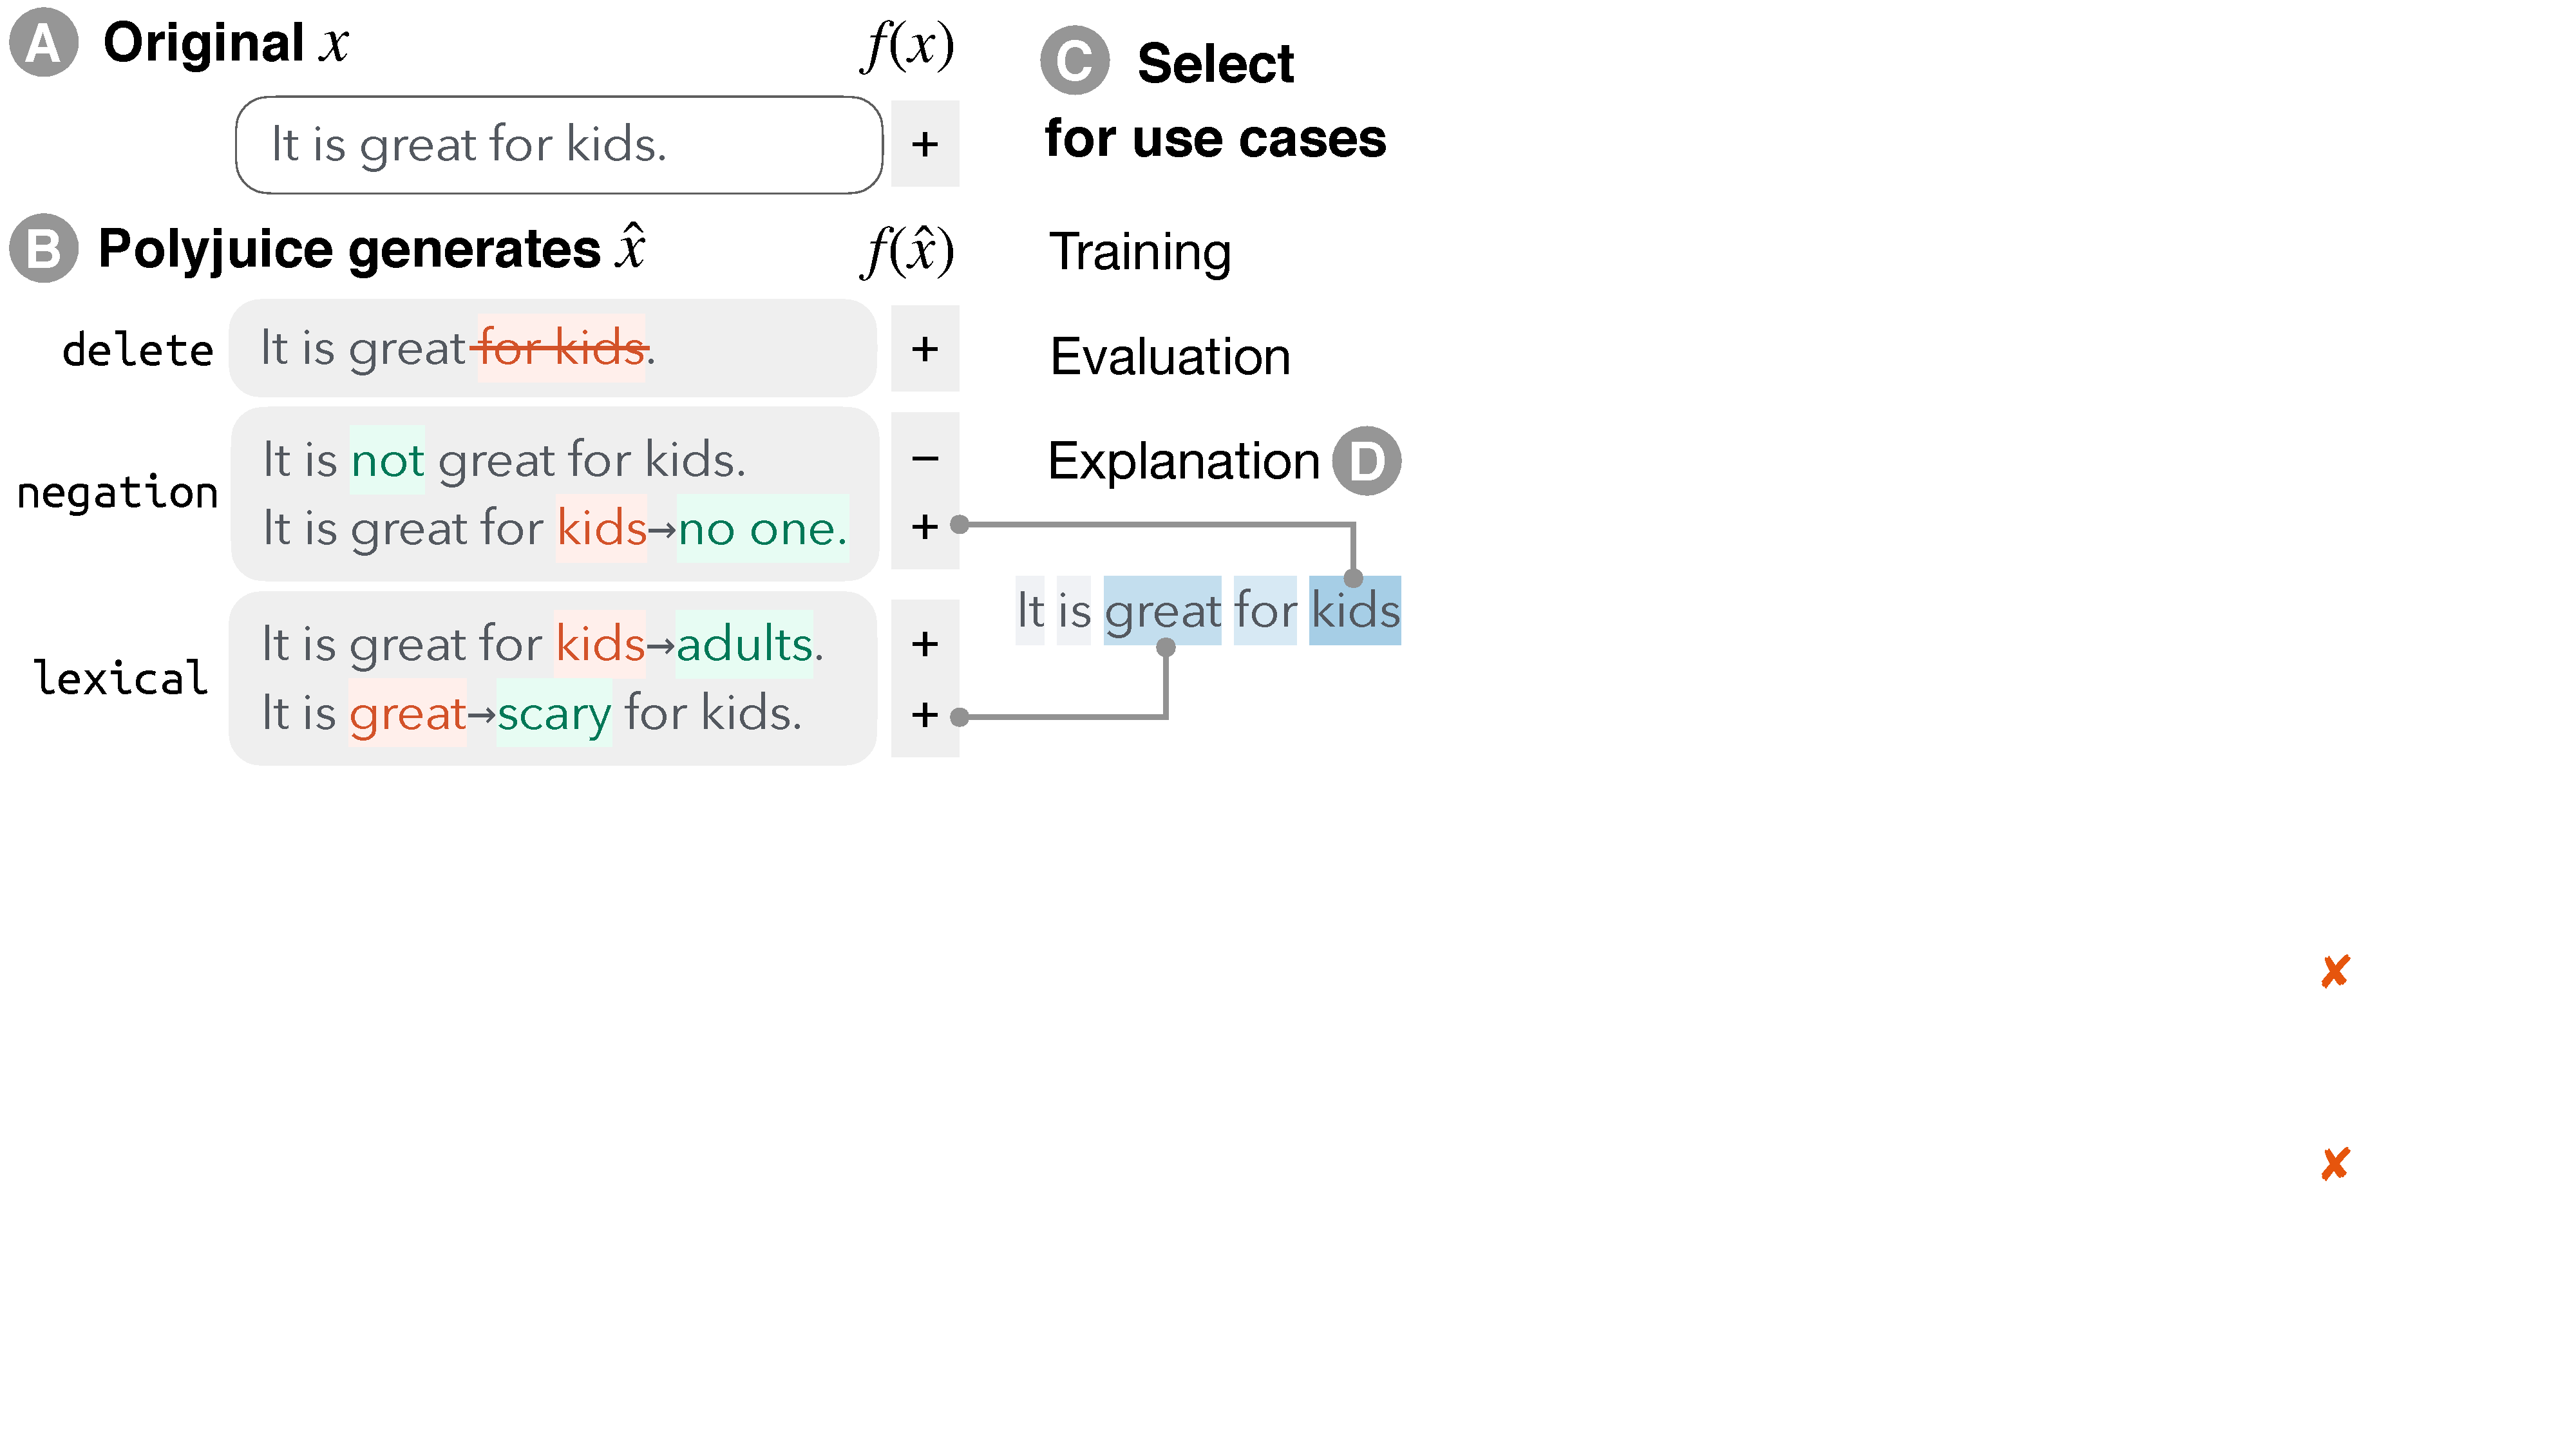
\includegraphics[trim={0 18cm 30.5cm 0cm},clip, width=1\columnwidth]{figures/teaser.pdf}
\vspace{-15pt}
\caption{
Overview: (A) given a sentiment analysis instance $x$, \sysname generates (B) various counterfactuals $\xp$, which are then (C) selected for downstream use.
\eg in (D) we select counterfactual explanations that complement a black box explanation: though ``great'' and ``kids'' are deemed important, perturbing them may not affect the prediction $f(x)=f(\xp)=\text{\emph{positive}}$, revealing model failures not covered by feature attributions.\footnotemark
}
\vspace{-10pt}
\label{fig:teaser}
\end{figure} 
\footnotetext{We open source both the \sysname model and the selection heuristics at \modelurl.}


%However, as Figure~\ref{fig:teaser} illustrates, counterfactual generation does not \emph{have} to be task-specific, as various applications share similar requirements on $x\veryshortarrow\xp$ (\eg a preference for small changes).
%In fact, a general-purpose pool of diverse counterfactuals may be preferable when the relationship is not precisely defined in advance, as is the case for counterfactual training, evaluation, or explanations.
% In fact, a common pool of counterfactuals may support each application more comprehensively.
% For example, without the preset constrain on semantic equivalence, we can collect adversarials through negation (for tasks insensitive to negation, \eg named entity recognition.)
%For example, some forms in training and evaluation data collection can 
%The exhaustive search of automated methods can cover the training and evaluation more comprehensively, and non-paraphrasing changes like \emph{add negation} are valuable adversarials for tasks like named entity recognition. 
%\hao{might be good to clarify that these two are not mutually-exclusive: adversarial examples should sometimes be close to the original}
% 
However, counterfactual generation does not \emph{have} to be task-specific.
The same set of counterfactuals in Figure~\ref{fig:teaser} can support a variety of applications.
Moreover, for cases like model explanation and analysis, a general-purpose pool of counterfactuals is preferable, as the relationship-of-interest can be more exploratory and user-oriented~\cite{wu2019errudite}.
In this work, we formalize the task of \emph{counterfactual generation}, disentangling generation from the application of counterfactuals (\S\ref{sec:general_purpose}).
Given an input $x$, our generator produces a set of counterfactuals $\hat{\xset} = \{\xp_1, \xp_2, ...\}$ with \emph{application-agnostic} relationships $x \veryshortarrow \xp_i$ (Figure~\ref{fig:teaser}B).
Afterwards, we use \emph{application-specific} selection methods to find subsets of $\xp$ that are most effective for a given use case (Figure~\ref{fig:teaser}C).

We frame the generation step as conditional text generation, and finetune GPT-2~\cite{radford2019language} into a generator called \emph{\sysname} using $(x, \xp)$ pairs. 
To allow for targeted counterfactuals, we also design \tagstrs like \ctrltag{negation} or \ctrltag{delete} (Figure~\ref{fig:teaser}B), and adopt fill-in-the-blank structures~\cite{donahue2020enabling} to specify where the perturbation occurs and how.
%We also allow for targeted counterfactuals, by specifying where the perturbation occurs~\cite{donahue2020enabling} and designing \tagstrs like \ctrltag{negation} or \ctrltag{delete} (Figure~\ref{fig:teaser}B).
Intrinsic evaluation shows that \sysname generates $\xp$ that are \emph{fluent}, \emph{diverse}, and \emph{close to $x$}, and that the \emph{control} mechanisms effectively retrieve perturbations that are rare to sample from off-the-shelf language models. %(\eg 42\% more negations).

%--- the control is \emph{the backbone of} various downstream applications.

%We propose simple yet effective selection strategies, 
With simple selection heuristics, we show that a single \sysname model can significantly aid humans in diverse downstream applications.\footnote{We demonstrate \sysname in semi-automatic settings, but as discussed in \S\ref{subsec:nlg}, it can also work automatically.} 
For \emph{counterfactual training and evaluation} (\S\ref{sec:app_label}), humans label \sysname counterfactuals rather than creating them from scratch.
They produce training data that significantly improves model generalization, as well as contrast sets that help identify model vulnerabilities~\cite{gardner2020contrast}, with 40--75\% less annotation effort. 
In another application, \sysname produces \emph{counterfactual explanations} (\S\ref{sec:app_explain}), bringing significant insight on top of state-of-the-art explanation techniques. 
Finally, \sysname supports counterfactual \emph{error analysis} (\S\ref{sec:app_err_analysis}).
It allows users to explore related counterfactuals (\eg the model responds differently to different negation forms in Figure~\ref{fig:teaser}B), and to aggregate individual counterfactuals into patterns, gaining systematic understanding of model behavior. 

%First, 
% By lifting the burden of manual rewrite, \sysname \emph{facilitates effective counterfactual training and evaluation}.
% With humans only \emph{labeling} counterfactuals, we produce training data that improves model generalization, as well as high-quality contrast sets~\cite{gardner2020contrast} with 40\%--75\% less annotation effort compared to creating them from scratch~\cite{kaushik2019learning}. 
%We similarly produce training data that improves model generalization in three classification tasks. %, when compared to adding the same amount of non-counterfactual data.

% (2) 
% %Second, 
% By generating nontrivial counterfactuals beyond paraphrasing and human intuitions, \sysname helps \emph{produce counterfactual explanations} that highlight model errors obscure to humans. 
% In a user study, experts only did slightly better than random (accuracy: $55 \pm 6\%$) at predicting what a model would do on \sysname counterfactuals, even after inspecting the model on their own.
% (3) 
% %Third, 
% By rewriting each instance in multiple ways, \sysname \emph{supports more systematic error analysis}.
% Case studies demonstrate that \sysname counterfactuals help contrast model behaviors on related perturbations (\eg the model in Figure~\ref{fig:teaser} responds differently to the two negation forms.)

% We opensource both the \sysname model and the selection strategies at \modelurl.


\begin{comment}
In summary, we:
\begin{compactenum}
\item Formalize the general-purpose counterfactual generation task. 
By \emph{separating the generation from the use cases}, we generate fluent and diverse counterfactuals that bypass application-specific constraints.
%. \hao{maybe emphasize the benefits of this}
\item Finetune a generator called \sysname, by collecting paired sentences and enhancing controls with infilling structures and \tagstrs --- the control is \emph{the backbone of} various downstream applications.
%\sysname generates plausible and diverse counterfactuals, with control over where perturbations happen and what they do.
The model is at \modelurl.
%, and we plan to opensource the selection strategies.
\item Apply \sysname to \emph{model training, evaluation, and explanation}, using various selection methods (which we will opensource).
\sysname helps collect high-quality training and evaluation data with 40\% less annotation effort, and find model bugs that on top of feature attribution explanations and counterfactual analysis.
\end{compactenum}
\wts{Maybe can delete if we run out of space.}
\end{comment}

% we observe that \sysname explanations can complement popular feature attribution methods and highlight their blind spots.
% After viewing SHAP weights~\cite{NIPS2017_7062} and interacting with the model, experts still could not predict model behaviors on counterfactuals selected for explanations, and missed 5\% and 25\% more cases than the human-generated or random baselines.


\bibliography{anthology,ref}
\bibliographystyle{acl_natbib}

\appendix

\end{document}
